\documentclass[11pt]{article}
\usepackage[margin=1in]{geometry}
\usepackage{amsmath,amssymb,amsfonts}
\usepackage{graphicx,float}
\usepackage{fancyhdr,booktabs}
\usepackage{listings}
\usepackage{hyperref}
\lstset{
    language=Matlab,
    basicstyle=\ttfamily\small,
    breaklines=true,
    keepspaces=true,
    showstringspaces=false
}

% Header and Footer Setup (following Homework 2)
\pagestyle{fancy}
\fancyhf{}
\lhead{ME 351 -- Fall 2026}
\rhead{Homework 4}
\cfoot{\thepage}

\title{\textbf{ME 351}\\[0.5ex]\Large Homework 4}
\author{Zeshui Song}
\date{Fall 2026}

\begin{document}
\maketitle
\vspace{-1em}

\subsection*{Exercise 1: Stability margins}
For the plant
\[
P(s)=\frac{1}{(s+1)(0.2s+1)(0.1s+1)},
\]
consider the three PI controllers
\[
C_1(s)=2.5\left(0.1+\frac{1}{s}\right),\qquad
C_2(s)=2.5\left(1+\frac{1}{s}\right),\qquad
C_3(s)=2.5\left(1+\frac{1}{10s}\right).
\]
The controllers are used to track a reference with negative unity feedback.
\begin{center}
    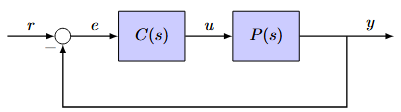
\includegraphics[width=0.65\linewidth]{ex1_block_diagram.png}
\end{center}

\paragraph{Part (a): Gain and phase margins (4 points)}
Find the gain and phase margins for all three controllers and illustrate them on appropriate Bode and Nyquist plots (Matlab allowed).\\\\
\textbf{Solution}\\
Using Matlab to compute the gain and phase margins, we have
\[
L_i(s)=C_i(s)P(s),\qquad i=1,2,3.
\]
\begin{lstlisting}
C1: GM = 7.60 dB, PM = 19.91 deg
C2: GM = 15.56 dB, PM = 53.41 deg
C3: GM = 17.76 dB, PM = 79.61 deg
\end{lstlisting}

\paragraph{Part (b): Closed-loop step response (5 points)}
Plot the three closed-loop step responses on the same axes, compare them, and identify the best controller. Explain what the Bode and Nyquist plots reveal about this comparison.
\newpage\noindent
\textbf{Solution}\par
\[
T_i(s)=\frac{L_i(s)}{1+L_i(s)}.
\]
Plotting on Matlab:
\begin{center}
    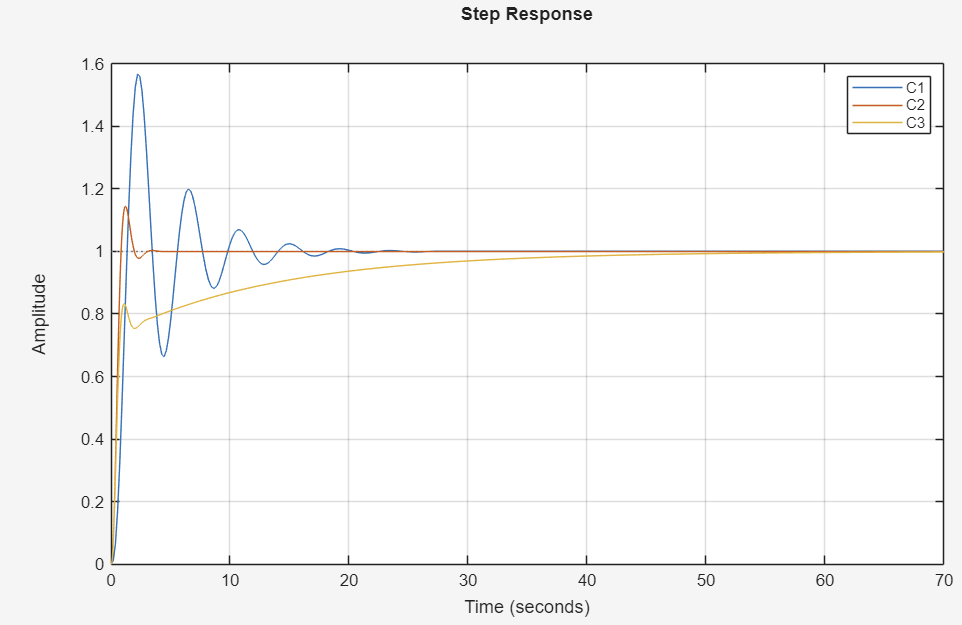
\includegraphics[width=0.8\linewidth]{1b step.png}
\end{center}
Generally, a smaller gain margin means less tolerance to additional controller gain before instability and smaller phase margin results in more overshoot and oscillation. A higher crossover frequency generally results in a faster response. 
\begin{center}
    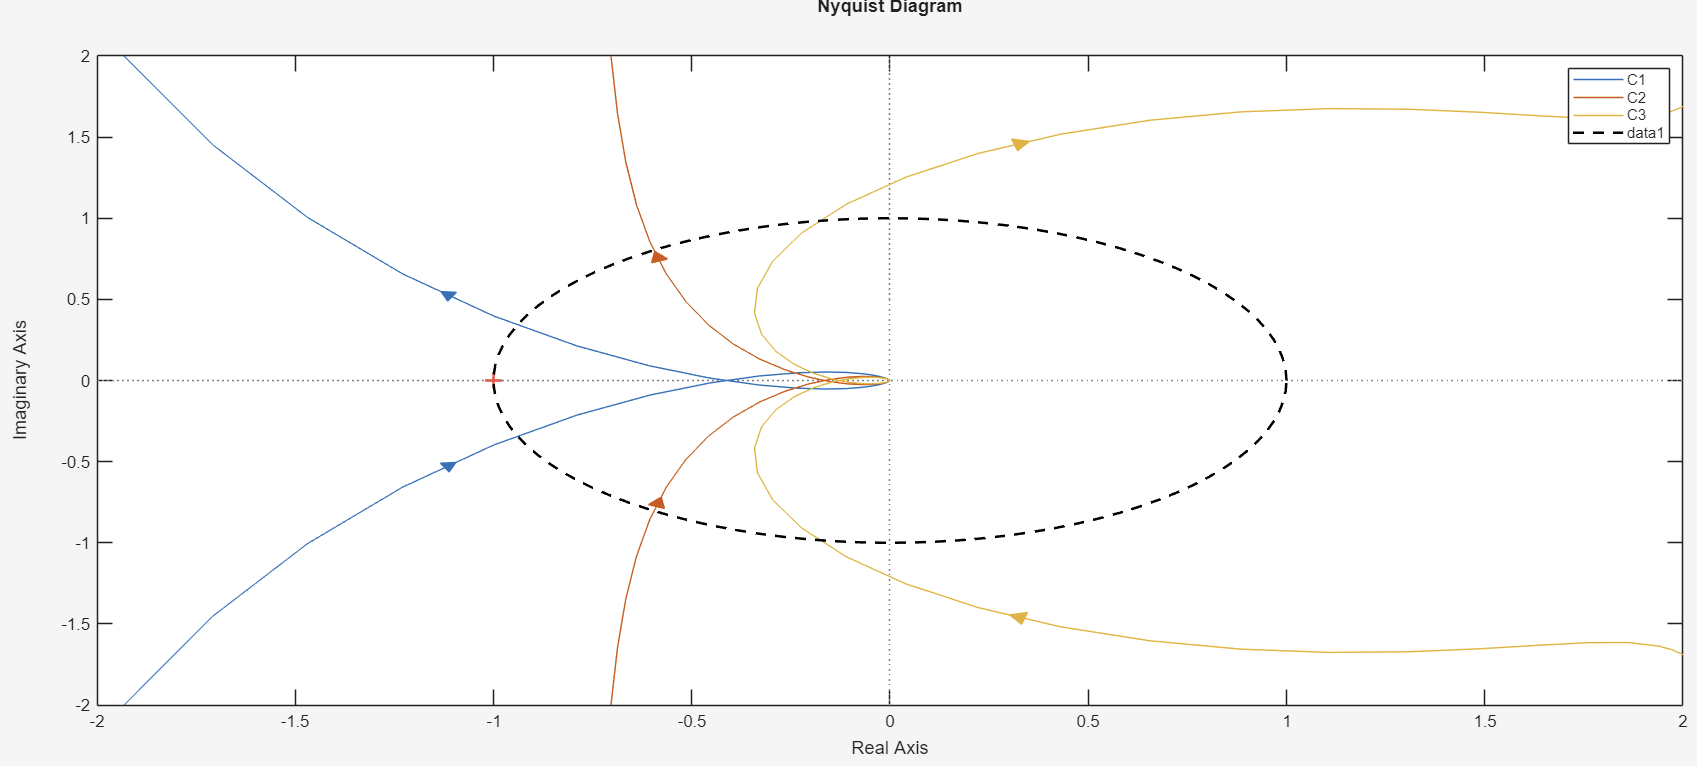
\includegraphics[width=0.8\linewidth]{1b nyquist.png}
\end{center}
From the nyquist plot:
\begin{itemize}
    \item When the plot intersects with the unit circle, it corresponds to a magnitude of 1 or 0 dB. This tells us the gain crossover frequency.
    \item When the plot intersects with the negative real axis, it corresponds to a phase of -180 degrees. This tells us the phase crossover frequency.
\end{itemize}
Thus, we can see that $C_1$ has the smallest phase margin, since it is closest in phase to the negative real axis when it intersects the unit circle.\\\\
Thus, $C_2$ is the best controller since it is sufficiently fast and has a good phase margin, while $C_3$ is too slow and $C_1$ is too oscillatory.
\subsection*{Exercise 2: Stability}
The following Nyquist plot and its zoom around the critical point describe an open-loop stable system.
\begin{center}
    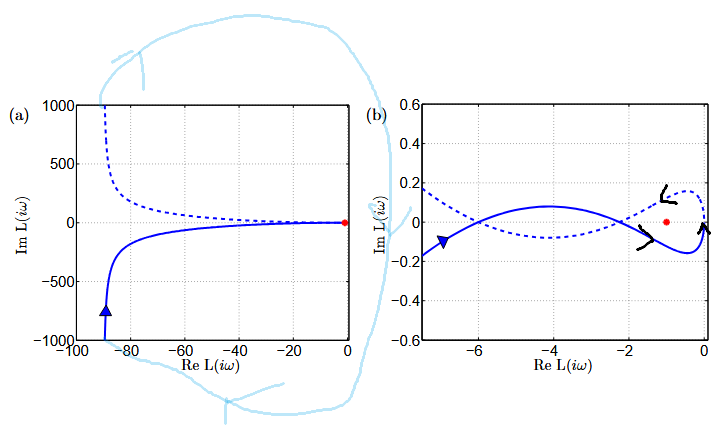
\includegraphics[width=0.8\linewidth]{ex2 nyquist.png}
\end{center}

\paragraph{Part (a): Closed-loop stability (2 points)}
Is the closed-loop system stable or unstable?\\\\
\textbf{Solution}\par
The fundamental nyquist equation is:
\[
\boxed{Z=N+P}
\]
Where:
\begin{itemize}
    \item $Z$: \# of RHP zeros of $1+L(s)$
    \item $N$: \# of clockwise encirclements of $(-1,0)$ by the Nyquist plot of $L(s)$. \textit{Counterclockwise encirclement adds -1}
    \item $P$: \# of RHP poles of $L(s)$
\end{itemize}
For the system to be stable, we need $Z=0$. Thus, given information that the open-loop system is stable, we have $P=0$. From there, we can count the number of encirclements to determine $Z$.\\\\
Because there is an integrator, the Nyquist plot starts from infinity in the zoomed out plot (a), but we can add a perturbation $\varepsilon$ to make it start from a finite point.\\\\
Counting the encirclements:
\begin{itemize}
    \item 1 larger clockwise encirclement of $(-1,0)$ in the zoomed out plot (a)
    \item 1 smaller counterclockwise encirclement of $(-1,0)$ in the zoomed in plot (b)
\end{itemize}
Thus, $N=1-1=0$.
\[\implies \boxed{Z=0}\]
Thus, the closed-loop system is stable.





\paragraph{Part (b): Varying the gain (4 points)}
Describe how stability changes as the gain increases from a very small to a very large value.\\\\
\textbf{Solution}\\
By increasing the gain, we are effectively increasing the distance of the Nyquist plot from the origin.\\\\
\textit{Recall that the Nyquist plot represents the magnitude and phase of the open-loop transfer function from the Bode plot in the complex plane, where each point corresponds to a specific $\omega$.}\\\\
Thus, eventually the ($-1,0$) point will be encircled by the middle loop in the zoomed in plot, thus resulting in $N=2$ and $Z=2$, which means the closed-loop system is unstable.
\begin{center}
    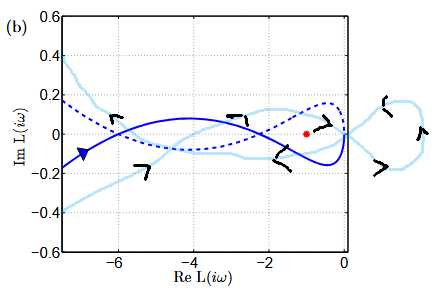
\includegraphics[width=0.5\linewidth]{2b.png}
\end{center}
\newpage
\paragraph{Part (c): Relative degree and root locus (4 points)}
Find the relative degree. Choose the corresponding root locus from the three given plots (a), (b), and (c), and explain why.
\begin{center}
    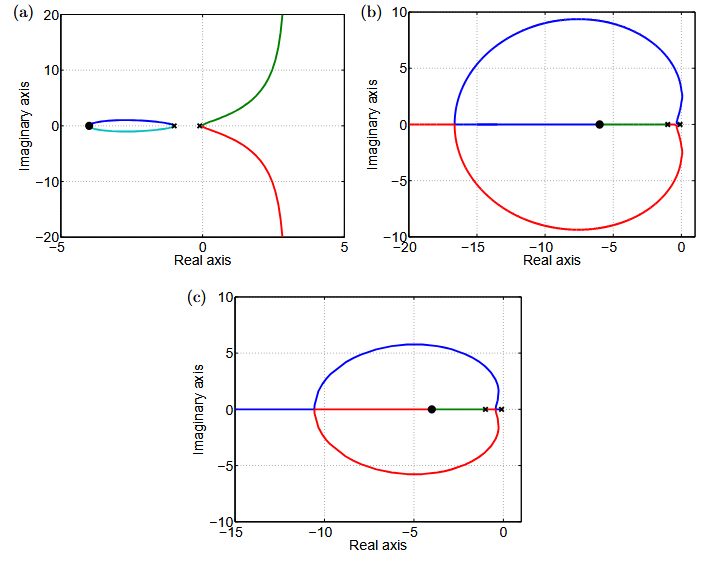
\includegraphics[width=0.8\linewidth]{ex2 root locus.png}
\end{center}
\textbf{Solution}\\
We can find the relative degree by looking at the high-frequency behavior of the nyquist plot as $\omega\to\infty$.\\\\
Suppose we have a loop transfer function with $n$ poles and $m$ zeros:
\[
L(s)=K\frac{(s+z_1)(s+z_2)\cdots(s+z_m)}{(s+p_1)(s+p_2)\cdots(s+p_n)}
\]
Evaluate for $s=j\omega$:
\[
L(j\omega)=K\frac{(j\omega+z_1)\cdots(j\omega+z_m)}{(j\omega+p_1)\cdots(j\omega+p_n)}
\]
For $\omega \gg z_i,p_i$:
\[
L(j\omega)\approx K\frac{(j\omega)^m}{(j\omega)^n}
\]
Thus, in terms of the relative degree $r=n-m$:
\[
\boxed{L(j\omega)\approx K(j\omega)^{-r}}
\]
Find the phase of $L(j\omega)$ for $K>0$:
\[
L(j\omega)\approx K(j\omega)^{-r} = \angle K\omega^{-r} + \angle (j^{-r}) = 0 - r\angle j = \boxed{-r(90^\circ)}
\]
Since the nyquist plot approaches $+90^\circ$ as $\omega\to\infty$, the relative degree is $r=3$ (the dotted line is for negative $\omega$, following the solid line, it asymptotes near the origin).\\\\
Since the relative degree is $3$, the root locus must have $3$ asymptotes, and so the \textbf{correct root locus is $A$.}
\paragraph{Part (d): Bode sketch (4 points)}
Sketch the corresponding Bode plot. Label key frequencies using pole and zero locations; numerical frequency values are not required.

\textbf{Solution}\par

\subsection*{Exercise 3: Controller design}
Consider a satellite attitude plant modeled by a double integrator:
\[
P(s)=\frac{1}{s^2}.
\]
The feedback loop tracks a reference angle, and the output may contain noise as indicated in the given diagram.
\begin{center}
    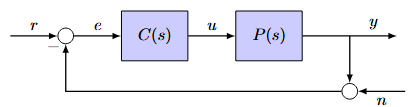
\includegraphics[width=0.65\linewidth]{ex 3 block diagram.png}
\end{center}

\paragraph{Part (a): Proportional feedback (2 points)}
Can proportional feedback stabilize the system? Justify with root-locus and Bode sketches (hand sketches preferred).

\textbf{Solution}\par
\[
C(s)=K_p.
\]

\paragraph{Part (b): Proportional-derivative feedback (4 points)}
Can a PD controller stabilize the system? Justify with root-locus and Bode sketches.

\textbf{Solution}\par
\[
C(s)=K_p+K_d s.
\]

\paragraph{Part (c): Proportional-integral feedback (4 points)}
Can a PI controller stabilize the system? Justify with root-locus and Bode sketches.

\textbf{Solution}\par
\[
C(s)=K_p+\frac{K_i}{s}.
\]

\paragraph{Part (d): Lead and lag compensation (4 points)}
For
\[
C(s)=k\frac{s+z}{s+p},
\]
with $k,z,p$ real (usually positive), compare a lead compensator ($0<z<p$) and a lag compensator ($0<p<z$). Sketch root locus and Bode plots for each and determine which can stabilize the plant.

\textbf{Solution}\par

\paragraph{Part (e): Frequency-domain design constraints (6 points)}
Sketch the constraints imposed on the loop-transfer-function Bode plot by:
\begin{enumerate}
    \item[(i)] zero steady-state error for a unit ramp, $R(s)=1/s^2$;
    \item[(ii)] less than $5\%$ steady-state error for sinusoidal reference inputs up to $1\,\mathrm{rad/s}$;
    \item[(iii)] output attenuation of noise above $100\,\mathrm{rad/s}$ by at least a factor of $10$.
\end{enumerate}

\textbf{Solution}\par

\paragraph{Part (f): Compensator design (8 points)}
Design a compensator meeting Part (e), with gain margin at least $2$ and phase margin at least $45^\circ$. Verify the design using Bode and Nyquist plots.

\textbf{Solution}\par
\[
C(s)=\boxed{\phantom{\dfrac{(s+1)(s+2)}{s(s+3)}}}.
\]

\paragraph{Part (g): Ramp simulation (2 points)}
Simulate the closed-loop response to a ramp and verify zero steady-state tracking error (Matlab \texttt{lsim} may be used).

\textbf{Solution}\par

\paragraph{Part (h): Sinusoidal simulation (2 points)}
Simulate the closed-loop response to $r(t)=\sin(t)$ and verify at most $5\%$ steady-state tracking error.

\textbf{Solution}\par

\end{document}
 